%---------------%
%->> Section 4.1: 系统架构
%------------%

\section{系统架构}

微服务故障诊断并不是固定流程下的顺序执行任务，而是一个由中间证据持续驱动的动态决策过程。任务开始时，系统通常只能获得告警信息、异常服务以及少量上下文；在后续诊断过程中，应优先检查哪些指标、日志或链路对象，是否继续沿当前路径深入，以及何时停止当前分支并转向其他可疑组件，都需要根据不断获得的新证据实时调整。与此同时，诊断过程还伴随着文件访问、命令执行、工具调用、状态记录和多轮任务推进等操作。因此，支撑该任务的平台不仅需要具备智能体运行能力，还需要提供面向工程环境的执行能力，以支持“边观察、边判断、边调整”的诊断过程。

基于上述特点，本文采用 OpenCode 作为故障诊断智能体平台的运行基础，而未将系统建立在传统智能体框架之上。一方面，OpenCode 作为开源平台，系统结构与执行链路较为透明，便于功能扩展、本地部署和实验复现；另一方面，OpenCode 原生支持多模型提供商与本地模型接入，可根据成本、时延和能力需求灵活切换模型。更重要的是，OpenCode 提供了 agent、subagent、skill、custom command 和 MCP server 等机制~\cite{opencode2025,claudecode_skills,mcp,luo2025mcpuniverse}，能够较好覆盖本文在任务拆分、角色分工、工具接入与执行控制等方面的实现需求。同时，其运行环境天然支持文件操作、命令执行和外部工具调用，更适合承载微服务故障诊断这类工具密集、路径动态变化的任务。

平台总体架构如图\ref{fig:system_architecture}所示。系统自上而下划分为前端展示层、Agent 执行层、Skill 组织层、MCP 接入层、后端服务层、数据存储层和外部服务层。前端展示层提供 Web 界面、SOP 可视化、故障指纹视图、诊断结果展示以及实时通信能力，用于支撑用户交互和任务状态反馈；Agent 执行层负责维护会话、加载 Skill、创建子代理并推进任务执行；Skill 组织层封装在线诊断、离线探索和规则整理三类核心任务；MCP 接入层将后端接口和观测能力以统一工具形式暴露给 Agent；后端服务层提供诊断任务 API、SOP 管理 API、故障指纹管理 API 以及数据查询 API；数据存储层保存 SOP 知识库、故障指纹库、执行轨迹和实验数据；外部服务层则负责提供大语言模型服务与监控数据源。各层通过标准接口衔接，形成了从前端交互、任务执行到结果持久化的完整链路。

\begin{figure}[htbp]
    \centering
    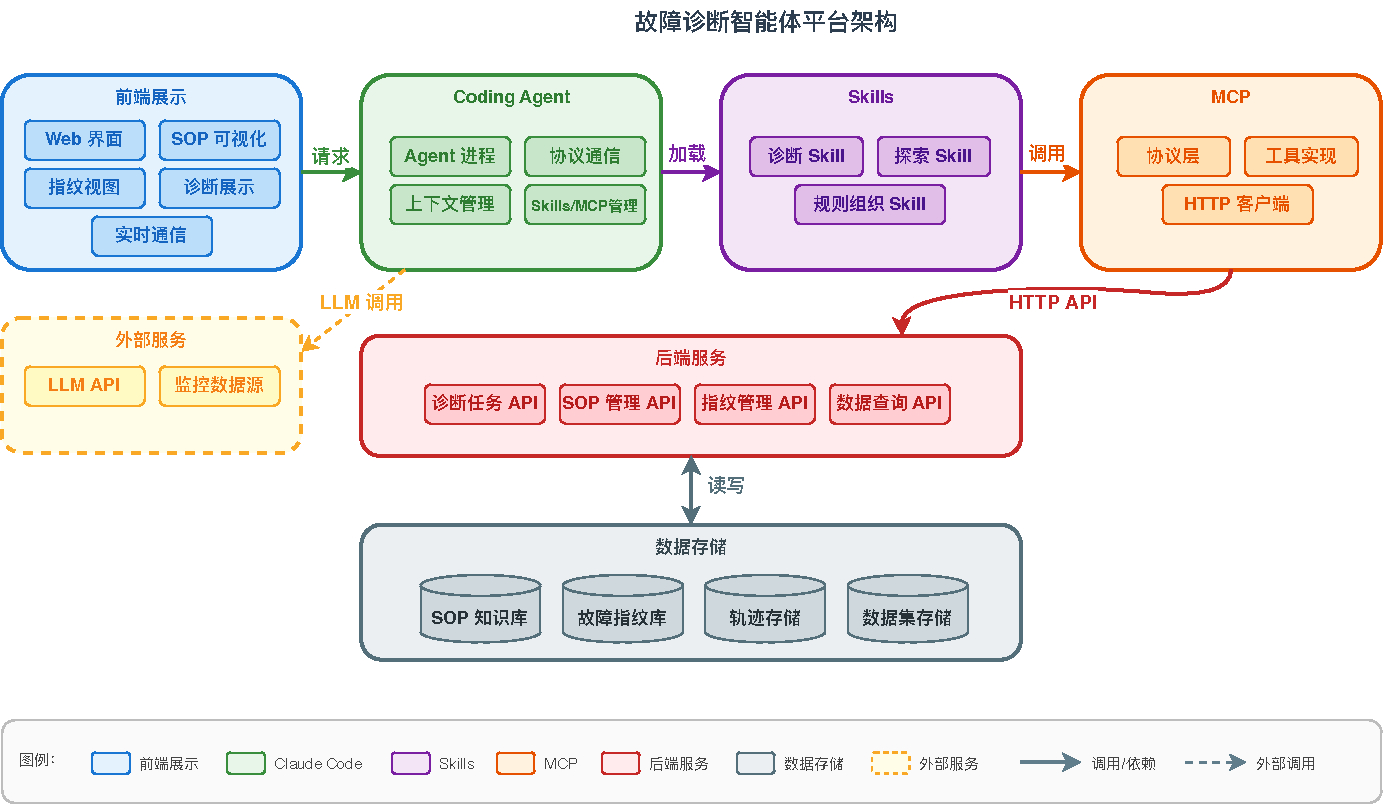
\includegraphics[width=\textwidth]{Figures-Src/Chap4-System/system-architecture/chart.pdf}
    \bicaption{基于 OpenCode 的微服务故障诊断平台架构}{Architecture of the Microservice Fault Diagnosis Platform Based on OpenCode}
    \label{fig:system_architecture}
\end{figure}

围绕第三章提出的方法，平台将系统中的核心任务进一步组织为 \texttt{Diagnosis-Skill}、\texttt{Exploration-Skill} 和 \texttt{Rule-Skill} 三类 Skill。其中，\texttt{Diagnosis-Skill} 面向告警驱动的在线诊断任务，负责读取告警信息、故障指纹检索结果和当前 SOP，并输出诊断结论与执行记录；\texttt{Exploration-Skill} 面向离线知识构建中的探索任务，围绕场景先验、可疑对象和现有 SOP 生成探索轨迹与补充证据；\texttt{Rule-Skill} 面向规则整理任务，读取探索轨迹与历史诊断记录，输出决策单元及更新后的 SOP。通过这种拆分方式，每个会话只加载与当前任务直接相关的约束、工具和上下文，从而避免不同任务逻辑在同一会话中相互干扰。

在平台中，Skill 用于组织任务目标与执行约束~\cite{claudecode_skills,claudecode-subagent}，MCP 用于接入具体能力~\cite{mcp,luo2025mcpuniverse,jayanti2026camcp,koc2025mcpide}。前者定义任务的输入输出形式、执行边界与行为规则，后者负责将后端接口和数据查询能力暴露为 Agent 可调用的统一工具。围绕这一分工，平台设置了 \texttt{Diagnosis MCP}、\texttt{Exploration MCP}、\texttt{Rule MCP} 和 \texttt{Observe MCP} 四类 MCP。其中，前三者分别服务于三类主任务，封装对应的操作说明、接口定义和结果返回方式；\texttt{Observe MCP} 则统一提供指标、日志、链路和感知域相关的查询能力。

指标查询、日志检索、链路分析以及感知域补充并未被进一步封装为独立的主 Skill，而是作为共享观测能力由各主任务按需调用。为此，平台引入观察子代理（Observe subagent）~\cite{claudecode-subagent}。当 \texttt{Diagnosis-Skill} 或 \texttt{Exploration-Skill} 在执行过程中需要补充观测证据时，主会话首先创建观察子代理，再由后者通过 \texttt{Observe MCP} 完成专项查询。主会话负责诊断推进、路径选择与状态维护，观察子代理负责围绕指定对象采集证据并返回结果。这样的组织方式不仅能够控制主会话的上下文规模，也使流程控制与证据采集相互分离，便于后续扩展新的观测能力。

从任务执行角度看，平台运行过程可概括为三个阶段。首先，用户通过前端发起在线诊断或离线知识构建请求，后端据此创建对应工作区并初始化场景上下文。其次，OpenCode 根据任务类型启动相应会话并加载对应 Skill：在线任务加载 \texttt{Diagnosis-Skill}，离线探索任务加载 \texttt{Exploration-Skill}，规则整理任务加载 \texttt{Rule-Skill}。最后，主 Skill 在运行过程中通过 MCP 调用后端接口；当需要补充观测证据时，再创建观察子代理，由其通过 \texttt{Observe MCP} 完成专项查询。执行过程中产生的轨迹、状态与结果持续同步至后端与数据存储层，并通过实时通信反馈到前端界面。经人工确认后的有效案例进一步回流至故障指纹库和 SOP 知识库，为后续离线更新提供输入，从而形成在线执行、结果沉淀与知识更新的闭环。

综上，本文基于 OpenCode 实现了面向微服务根因定位的故障诊断智能体平台。该平台以 Skill 承担在线诊断、离线探索和规则整理三类主任务，以 MCP 连接后端能力与观测工具，并通过观察子代理完成专项证据采集。整体架构能够适应微服务故障诊断中路径动态、工具密集和知识持续更新的任务特点，为后续在线诊断与离线知识演化提供统一的平台支撑。